\chapter{Miglioria dell'algoritmo di schedulazione}\label{chp:miglioria}
Nelle sezioni che seguono vengono ripercorsi i passi dell'algoritmo seguito nei capitoli precedenti, al fine di presentare le differenze introdotte a seguito dell'adozione del nuovo meccanismo di schedulazione.
\section{Presentazione del caso di studio}\label{sec:miglioria-presentazione}
La descrizione del caso di studio rimane pressoché inalterata, ad eccezione della presenza di alcune regole addizionali per la scelta dei ticket da servire.

Definiti:
\begin{itemize}
\item $A$ un cliente titolare di un conto \textsl{BancoPosta}, possessore di un ticket di tipo \uo{} o \pp{}.
\item $B$ un cliente \textbf{non} titolare di un conto \textsl{BancoPosta}, possessore di un ticket di tipo \uo{} o \pp{}.
\item $C$ un cliente possessore di un ticket di tipo \sr{}.
\end{itemize}
Di seguito, sono riportate le regole aggiuntive:
\begin{itemize}
\item Dopo ogni cliente di tipo $A$ servito, gli sportelli non dedicati servono, se presente, uno di tipo $B$, privilegiando la fila più lunga. 
\item Dopo ogni 4 clienti di tipo $C$ serviti, lo sportello dedicato serve, se presente, uno di tipo $B$, privilegiando la fila più lunga.
\item Nel caso in cui non vi siano clienti di tipo $C$ da servire, lo sportello dedicato dà priorità a quelli di tipo $B$, privilegiando la fila più lunga.
\end{itemize}
\section{Obiettivi dello studio}\label{sec:miglioria-obiettivi}
L'obiettivo di questo studio migliorativo è quello di diminuire, rispetto ai risultati precedentemente ottenuti, il numero degli sportelli da mantenere operativi in un'intera giornata lavorativa, continuando a garantire il rispetto dei requisiti di qualità stabiliti nel capitolo \ref{chp:obiettivi}.
\section{Modello concettuale}\label{sec:miglioria-modello-concettuale}
Il modello concettuale proposto nel capitolo \ref{chp:modello-concettuale} continua ad essere rappresentativo anche a seguito dell'introduzione della miglioria. 

Pertanto:
\begin{itemize}
\item Le variabili che descrivono univocamente, ad ogni istante di tempo, lo stato del sistema
\item Le assunzioni alla base del modello concettuale
\end{itemize}
sono le medesime introdotte in tale capitolo.
\section{Modello delle specifiche}\label{sec:miglioria-modello-specifiche}
Dal modello delle speficiche descritto nel capitolo \ref{chp:modello-specifiche}:
\begin{itemize}
\item Le variabili matematiche e le equazioni che le legano
\item Le assunzioni di base
\item I parametri di input del sistema
\end{itemize}
rimangono validi anche a seguito dell'introduzione della miglioria.

Considerando le regole di schedulazione addizionali espresse nella sezione \ref{sec:miglioria-presentazione}, gli algoritmi \ref{alg:modello-specifiche-1} e \ref{alg:modello-specifiche-2} sono stati rivisitati, applicando le opportune patch, come mostrato in \ref{alg:miglioria-modello-specifiche-1} e \ref{alg:miglioria-modello-specifiche-2}.

\begin{algorithm}[ht]
\SetAlgoLined
\While{true}{
\textcolor{purple}{\uIf{1 of `\uo{} \textsl{BancoPosta}' or `\pp{} \textsl{BancoPosta}' served}{
		\textit{pick the longest queue between `\uo{} \textsl{Standard}' or `\pp{} \textsl{Standard}'}\;
		\textit{processes the first ticket inside that queue}\;
	}}
	\uElseIf{`\uo{} \textsl{BancoPosta}' queue not empty}{
		\textit{processes the first ticket of that type}\;
	}
	\uElseIf{`\pp{} \textsl{BancoPosta}' queue not empty}{
		\textit{processes the first ticket of that type}\;
	}
	\uElseIf{`\uo{} \textsl{Standard}' queue not empty}{
		\textit{processes the first ticket of that type}\;
	}
	\uElseIf{`\pp{} \textsl{Standard}' queue not empty}{
		\textit{processes the first ticket of that type}\;
	}
	\uElse {
		\textit{do nothing}\;	
	}	
}
\caption{Algoritmo di schedulazione del servente generico (con {\color{purple}patch})}
\label{alg:miglioria-modello-specifiche-1}
\end{algorithm}

\begin{algorithm}
\SetAlgoLined
\While{true}{
	\textcolor{purple}{\uIf{4 of `\sr{} \textsl{BancoPosta}' or `\sr{} \textsl{Standard}' served}{
		\textit{pick the longest queue between `\uo{} \textsl{Standard}' or `\pp{} \textsl{Standard}'}\;
		\textit{processes the first ticket inside that queue}\;
	}}
	\uElseIf{`\sr{} \textsl{BancoPosta}' queue not empty}{
		\textit{processes the first ticket of that type}\;
	}
	\uElseIf{`\sr{} \textsl{Standard}' queue not empty}{
		\textit{processes the first ticket of that type}\;
	}
	\textcolor{purple}{\uElseIf{`\uo{} \textsl{Standard}' or `\pp{} \textsl{Standard}' queues are not empty}{
		\textit{pick the longest queue between them}\;
		\textit{processes the first ticket inside that queue}\;
	}}
	\uElseIf{`\uo{} \textsl{BancoPosta}' queue not empty}{
		\textit{processes the first ticket of that type}\;
	}
	\uElseIf{`\pp{} \textsl{BancoPosta}' queue not empty}{
		\textit{processes the first ticket of that type}\;
	}
	\uElse {
		\textit{do nothing}\;	
	}
}
\caption{Algoritmo di schedulazione del servente dedicato (con {\color{purple}patch})}
\label{alg:miglioria-modello-specifiche-2}
\end{algorithm}

\section{Modello computazionale}\label{sec:miglioria-modello-computazionale}
Dal modello computazionale descritto nel capitolo \ref{chp:modello-computazionale}:
\begin{itemize}
\item Le variabili di programma (sez. \ref{sec:modello-computazionale-stato})
\item Gli eventi (sez. \ref{sec:modello-computazionale-eventi})
\item Il clock di simulazione (sez. \ref{sec:modello-computazionale-clock})
\item Scheduler (sez. \ref{sec:modello-computazionale-scheduler})
\item Lista degli eventi (sez. \ref{sec:modello-computazionale-lista-eventi})
\item Generazione dei nuovi eventi (sez. \ref{sec:modello-computazionale-gen-nuovi-eventi})
\item Campionamento delle statistiche (sez. \ref{sec:modello-computazionale-campionamento-stat})
\end{itemize}
rimangono validi anche a seguito dell'introduzione della miglioria.

\subsection{Algoritmo next-event}
Per la realizzazione della miglioria, a livello di codice, sono state definite due ulteriori variabili:
\begin{itemize}
\item \texttt{{\color{code_purple}int} counter\_served\_gen\_bp}: valore intero modulo 2, utilizzato per mantenere il numero di clienti afferenti alle classi \uo{} \textsl{BancoPosta} e \pp{} \textsl{BancoPosta} serviti dagli sportelli generali.
\item \texttt{{\color{code_purple}int} counter\_served\_sr}: valore intero modulo 5, utilizzato per mantenere il numero di clienti afferenti alle classi \sr{} \textsl{BancoPosta} e \sr{} \textsl{Standard} serviti dallo sportello dedicato.
\end{itemize}

I passi di \textit{inizializzazione}, \textit{processamento dell'evento corrente} e \textit{terminazione} dell'algoritmo di simulazione rimangono inalterati rispetto a quanto descritto nella \ref{sec:modello-computazionale-algoritmo}. Di seguito è riportato lo step della \textit{schedulazione di nuovi eventi} le cui modifiche sono evidenziate in {\color{purple}viola}:
\begin{enumerate}[label=Step \arabic*), align=left, leftmargin=*]
\setcounter{enumi}{2}
\item \textbf{Schedulazione nuovi eventi}
\begin{itemize}
\item Nel caso in cui l'evento corrente sia un arrivo di un cliente afferente ad una classe $c$ ed esiste un servente libero in grado di servirlo:
\begin{enumerate}
\item Lo stato del servente viene posto pari ad \texttt{1} (\texttt{BUSY}).
\item Il numero di clienti in servizio afferenti alla classe $c$ viene incrementato di una unità.
\item Viene generato l'istante di completamento di tale servizio, come descritto nella sezione \ref{sec:modello-computazionale-gen-nuovi-eventi}.
\end{enumerate}

\item Nel caso in cui l'evento corrente sia un completamento di un cliente afferente alla classe:
{\color{purple}
\begin{itemize}
\item \uo{} \textsl{BancoPosta} o \pp{} \textsl{BancoPosta}, da parte di un servente generale, si incrementa, in modo modulare, il contatore \texttt{counter\_served\_gen\_bp}.
\item \sr{} \textsl{BancoPosta} o \sr{} \textsl{Standard}, si incrementa, in modo modulare, il contatore \texttt{counter\_served\_sr}.
\end{itemize} 
Inoltre,} il servente che si è appena liberato processa, se presente, il primo cliente in coda seguendo l'ordine di priorità\footnote{È opportuno ricordare che tale ordine è diverso da quello del sistema originale, in accordo a quanto descritto nella sezione \ref{sec:miglioria-presentazione} e negli algoritmi \ref{alg:miglioria-modello-specifiche-1} e \ref{alg:miglioria-modello-specifiche-2}.}, replicando i punti (a), (b) e (c) del bullet dedicato all'arrivo di un nuovo cliente.
\end{itemize}

\end{enumerate}

\section{Verifica}\label{sec:miglioria-verifica}
Per poter controllare che tutte le modifiche introdotte con la miglioria operassero come atteso, seguendo lo stesso approccio adottato nel capitolo \ref{chp:verifica}, è stata utilizzata la funzione \texttt{print\_update()}, modificata al fine di mostrare:
\begin{itemize}
\item Il numero intero modulo $2$ di ticket \uo{}	\textsl{BancoPosta} e \pp{} \textsl{BancoPosta} serviti.
\item Il numero intero modulo $5$ di ticket \sr{} serviti.
\end{itemize}

\subsection{Controlli di consistenza sullo scheduler}
I controlli di consistenza effettuati sullo scheduler, che fanno riferimento alle porzioni in {\color{purple} viola} dei modelli delle specifiche (sez. \ref{sec:miglioria-modello-specifiche}) e computazionale (sez. \ref{sec:miglioria-modello-computazionale}), sono di seguito analizzati:
\begin{itemize}
\item In figura \ref{fig:miglioria-verifica-1a} è mostrata una verifica di come, dopo che un servente generale completa il servizio di un cliente afferente alla classe d'utenza \uo{} \textsl{BancoPosta}, ne serve uno non titolare di conto \textsl{BancoPosta} appartente alla coda più lunga (evidenziato in {\color{verify_blue}blu}), ovvero \uo{} \textsl{Standard} (evidenziato in {\color{verify_red}rosso}). 

Inoltre, è possibile osservare come il contatore venga correttamente azzerato (evidenziato in {\color{verify_yellow}giallo}).
\item In figura \ref{fig:miglioria-verifica-1b} è mostrata una verifica di come, dopo che il servente dedicato ha servito $4$ clienti in possesso di ticket \sr{}, ne serve uno non titolare di conto \textsl{BancoPosta} appartente alla coda più lunga (evidenziato in {\color{verify_blue}blu}), ovvero \pp{} \textsl{Standard} (evidenziato in {\color{verify_red}rosso}). 

Inoltre, è possibile osservare come il contatore venga correttamente azzerato (evidenziato in {\color{verify_yellow}giallo}).
\item In figura \ref{fig:miglioria-verifica-2} è mostrata una verifica di come, in assenza di ticket \sr{} da servire (evidenziato in {\color{verify_yellow}giallo}), lo sportello dedicato serve un cliente non titolare di conto \textsl{BancoPosta} appartente alla coda più lunga (evidenziato in {\color{verify_blue}blu}), ovvero \uo{} \textsl{Standard} (evidenziato in {\color{verify_red}rosso}).
\end{itemize}

In particolare, gli screenshot riportati nelle figure \ref{fig:miglioria-verifica-1}, \ref{fig:miglioria-verifica-2} e \ref{fig:miglioria-verifica-3}, e sopra più volte referenziati, sono stati tutti quanti realizzati fissando come seed iniziale \texttt{10}.

\begin{figure}[ht]
\centering
\captionsetup[subfigure]{justification=centering}
\begin{subfigure}[b]{0.475\textwidth}
\centering 
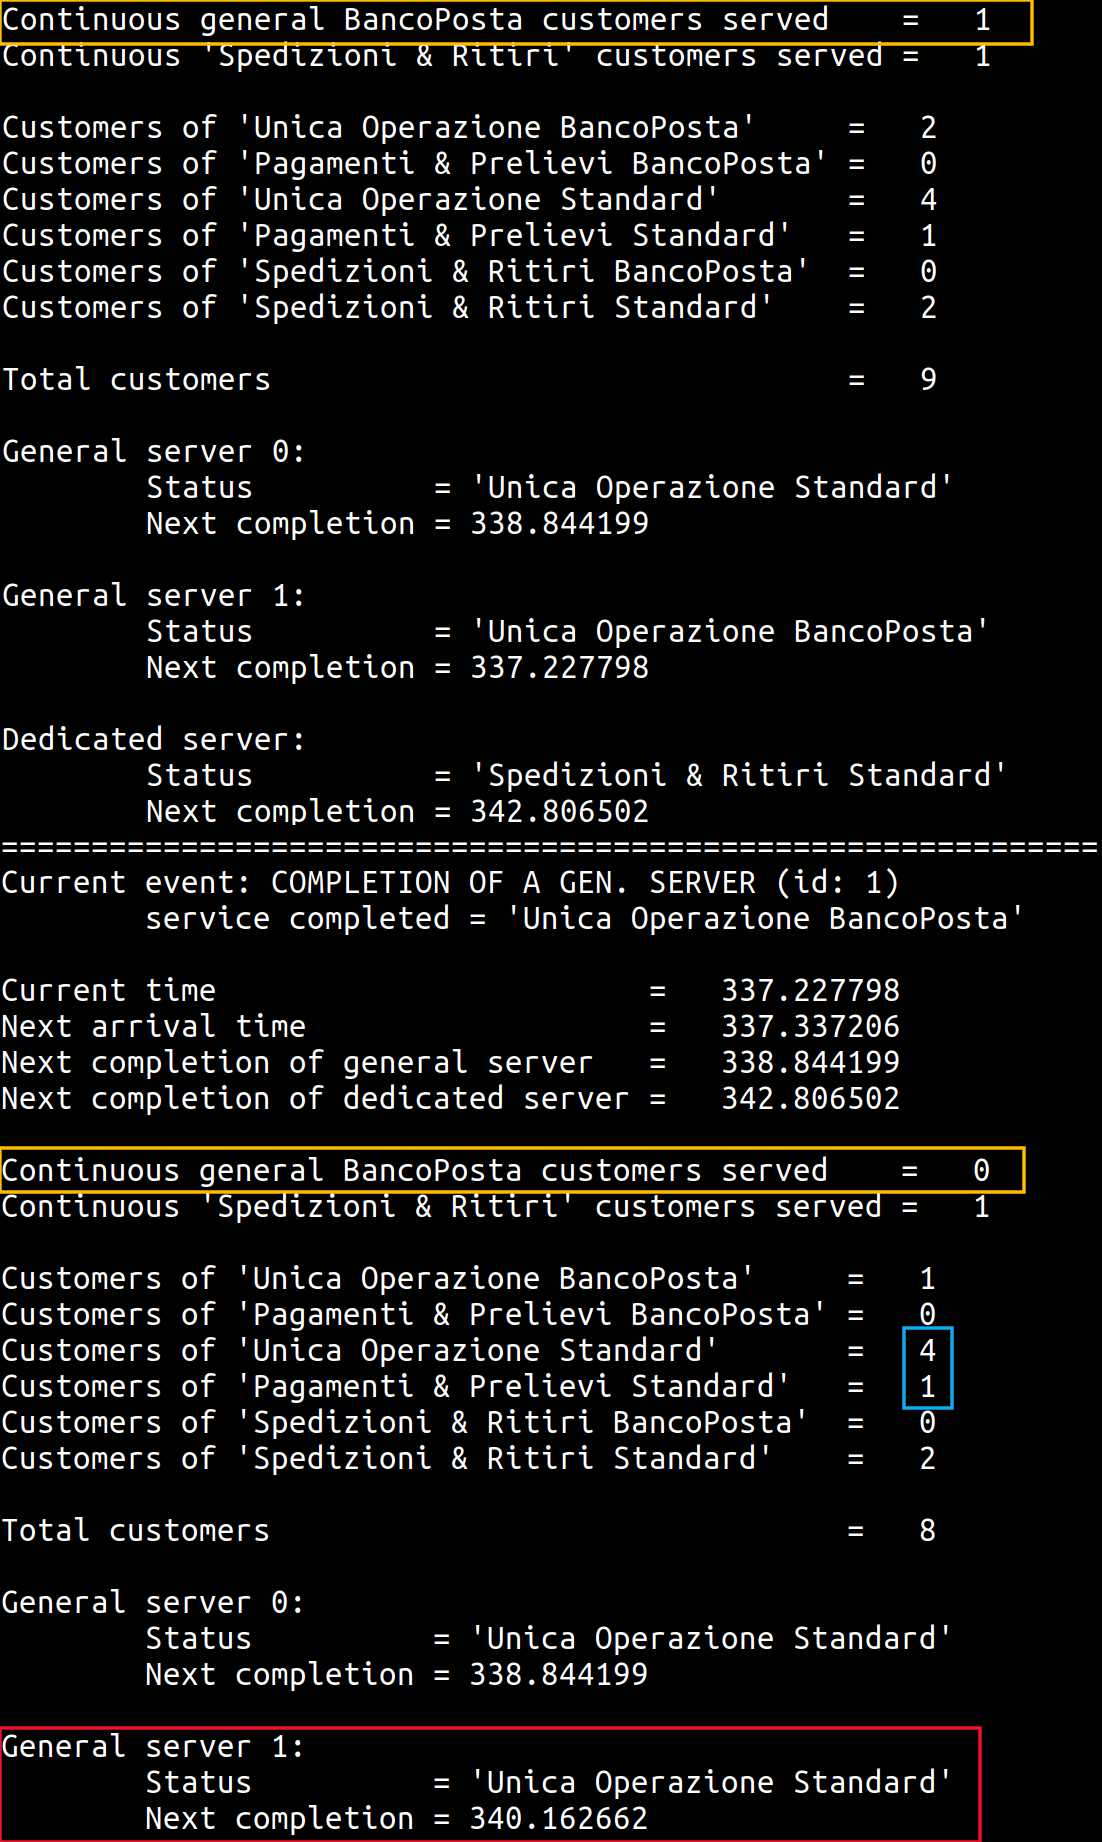
\includegraphics[width=\textwidth]{screenshots/improved/exception_gen}
\caption{Il servente generale processa un ticket non \textsl{BancoPosta}}   
\label{fig:miglioria-verifica-1a}
\end{subfigure}
\hfill
\begin{subfigure}[b]{0.475\textwidth}   
\centering 
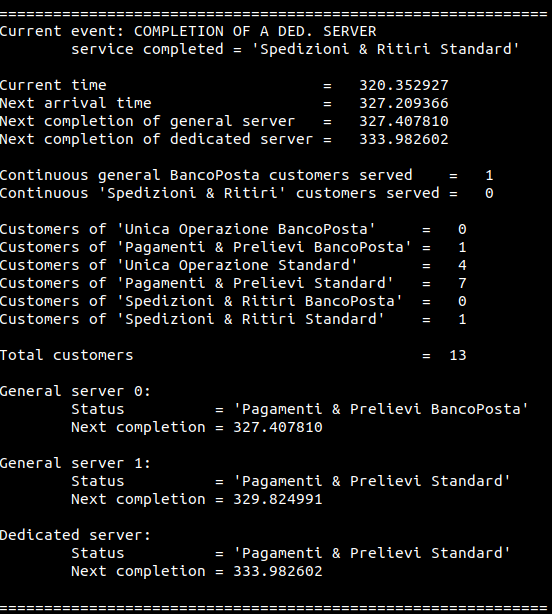
\includegraphics[width=\textwidth]{screenshots/improved/exception_ded}
\caption{Il servente dedicato processa un ticket \uo{} o \pp{} \textbf{non} \textsl{BancoPosta}}    
\label{fig:miglioria-verifica-1b}
\end{subfigure}
\caption{Verifica del corretto cambiamento della priorità a seguito del raggiungimento della soglia}
\label{fig:miglioria-verifica-1}
\end{figure}

\captionsetup[figure]{justification=centering}
\begin{figure}[ht]
\centering
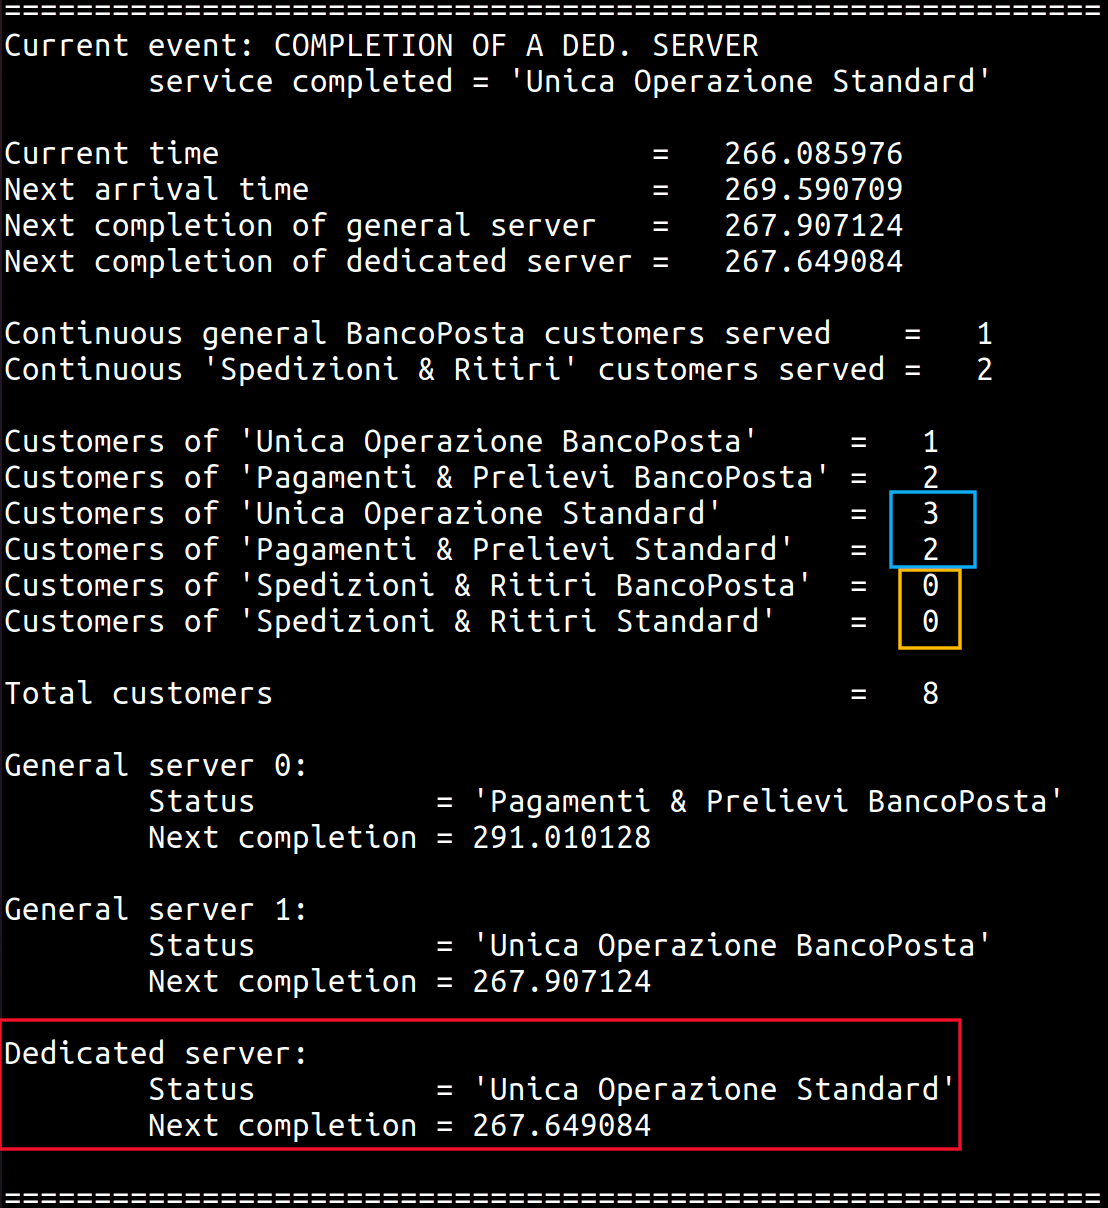
\includegraphics[width=0.5\textwidth]{screenshots/improved/longest_queue_ded_no_SR}
\caption{In assenza di \sr{}, lo sportello dedicato serve un cliente non titolare di conto \textsl{BancoPosta} appartenente alla coda più lunga}   
\label{fig:miglioria-verifica-2}
\end{figure}

\section{Controlli di consistenza sulle statistiche di output}
Di seguito vengono effettuati i controlli di consistenza sulle statistiche di output:
\begin{itemize}
\item Per le statistiche job-averaged, per definizione, si ha:
\begin{equation}
\bar{d} = \bar{w} - \bar{s}
\end{equation}
Dalla figura \ref{fig:verifica-2} è facile osservare che questa relazione sia rispettata. Ad esempio, per la classe d'utenza \uo{} \textsl{BancoPosta} vale che $\mathtt{10.47 - 6.51 = 3.96}$.
\item Per le statistiche time-averaged, per definizione, si ha:
\begin{equation}
\bar{q} = \bar{l} - \bar{y}
\end{equation}
Dalla figura \ref{fig:verifica-2} è facile osservare che questa relazione sia rispettata. Ad esempio, per la classe d'utenza \uo{} \textsl{BancoPosta} vale che $\mathtt{0.33 - 0.21 = 0.12}$.
\item Dalla teoria è noto che:
\begin{equation}
\begin{array}{c c c}
\bar{l} = \frac{n}{c_n} \cdot \bar{w}, & \bar{q} = \frac{n}{c_n} \cdot \bar{d}, & \bar{y} = \frac{n}{c_n} \cdot \bar{s} 
\end{array}
\end{equation}
Dalla figura \ref{fig:verifica-2} è facile osservare che questa relazione sia rispettata. Ad esempio, per la classe d'utenza \pp{} \textsl{Standard} vale che $\mathtt{\frac{32}{538.25} \cdot 16.49 = 0.980362 \simeq 0.98}$.
\end{itemize}

\begin{figure}[ht]  
\centering 
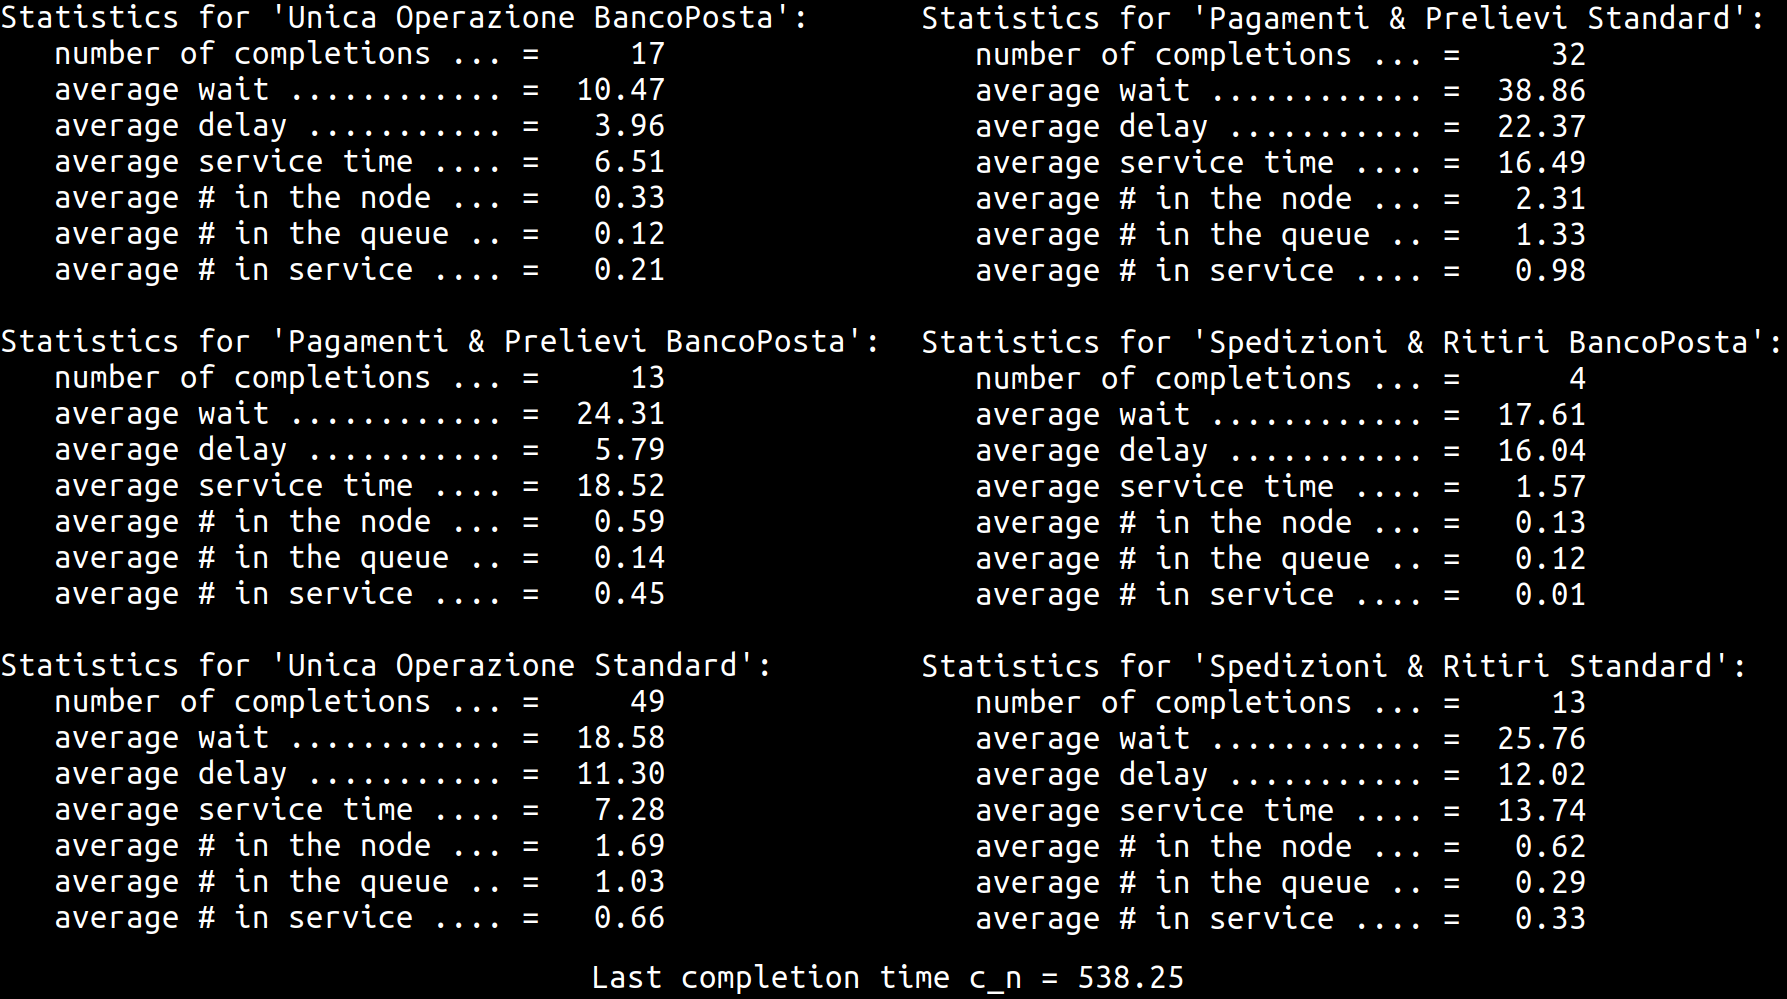
\includegraphics[width=\textwidth]{screenshots/improved/statistics}
\caption{Statistiche per ciascuna classe di utenza computate su un singolo run}   
\label{fig:miglioria-verifica-3}
\end{figure}

\section{Validazione}\label{sec:miglioria-validazione}
Per la fase di validazione, è stato seguito lo stesso approccio mostrato nel capitolo \ref{chp:validazione}. Per semplicità, di seguito è riportata la configurazione dei parametri utilizzati per la simulazione:
\begin{itemize}
\item \texttt{B = 256}
\item \texttt{K = 64}
\item \texttt{STOP = 16384}
\item \texttt{STAT\_INIT\_SEED = 12345}
\end{itemize}
Inoltre, è stato utilizzato il programma \texttt{estimate} per il calcolo delle realizzazioni degli intervalli di confidenza al 95\%.

\newpage
\subsection{Blocco del flusso degli arrivi di tipo \sr{} e innalzamento valore soglia}
Privando il sistema della generazione di arrivi di tipo \sr{}, come mostrato in figura \ref{fig:validazione-semplificazione-1}, e inoltre:
\begin{itemize}
\item Fissando $M = 3$
\item Disabilitando il meccanismo introdotto dalla miglioria per i serventi generali, ovvero innalzando il valore soglia per il contatore \texttt{counter\_served\_gen\_bp} a 1000
\end{itemize}
si ottengono i seguenti risultati:
\begin{itemize}
\item Mediante la simulazione:
\begin{itemize}
\item Un intervallo di confidenza al 95\% per il tempo medio d'attesa globale è pari a:
\begin{equation} 
\bar{d}_g = \sum_{i = 1}^4 p_{g,i}\cdot \bar{d}_{g,i} = (4.35 \pm 1.04)\ min
\end{equation}
\item Un intervallo di confidenza al 95\% per il tempo medio di risposta globale è pari a:
\begin{equation}
\bar{w}_g = \sum_{i = 1}^4 p_{g,i}\cdot \bar{w}_{g,i} = (14.66 \pm 1.31)\ min
\end{equation}
\end{itemize}

\item Mediante l'analisi effettuata in riferimento al modello a code riportato in figura \ref{fig:validazione-modello-analitico-1a}:
\begin{itemize}
\item Il tempo medio d'attesa globale ottenuto è pari a:
\begin{equation}
E[T_{Q_g}]^{KP} = 9.256825\ min 
\end{equation}
\item Il tempo medio di risposta globale ottenuto è pari a:
\begin{equation}
E[T_{S_g}] = 12.756807\ min 
\end{equation}
\end{itemize}
in accordo rispettivamente alle equazioni \ref{eqn:validazione-11} e \ref{eqn:validazione-13}.
\end{itemize}

I risultati ottenuti sono molto vicini a quelli della sezione \ref{sec:validazione-blocco-sr}, il che è ragionevole in quanto l'unica variazione tra il sistema privo di miglioria e quello in questione è dovuta al comportamento del server dedicato: la priorità maggiore è data alle richieste appartenenti alla coda più lunga tra quelle relative alla classe \uo{} \textsl{Standard} e \pp{} \textsl{Standard}.

Poiché, anche in questo caso, un intervallo di confidenza al 95\% per l'occupazione media ottenuta tramite la simulazione è pari a:
\begin{equation}
\bar{x}_g = 0.69 \pm 0.03
\end{equation}
si ritengono ragionevoli i risultati ottenuti per i motivi descritti nella sezione \ref{sec:validazione-blocco-sr}.

\subsection{Blocco del flusso degli arrivi di tipo \uo{} e \pp{}}
Privando il sistema della generazione di arrivi di tipo \uo{} e \pp{}, come mostrato in figura \ref{fig:validazione-semplificazione-2} e fissando $M = 4$, si ottengono i seguenti risultati:
\begin{itemize}
\item Mediante la simulazione:
\begin{itemize}
\item Un intervallo di confidenza al 95\% per il tempo medio d'attesa globale è pari a:
\begin{equation} 
\bar{d}_d = p_{d,1}\cdot \bar{d}_{d,1} + p_{d,2}\cdot \bar{d}_{d,2} = (6.04 \pm 1.88)\ min
\end{equation}
\item Un intervallo di confidenza al 95\% per il tempo medio di risposta globale è pari a:
\begin{equation}
\bar{w}_d = p_{d,1}\cdot \bar{w}_{d,1} + p_{d,2}\cdot \bar{w}_{d,2} = (16.45 \pm 2.64)\ min
\end{equation}
\end{itemize}

\item Mediante l'analisi effettuata in riferimento al modello a code riportato in figura \ref{fig:validazione-modello-analitico-1b}:
\begin{itemize}
\item Il tempo medio d'attesa globale ottenuto è pari a:
\begin{equation}
E[T_{Q_d}]^{KP} = 5.769637\ min 
\end{equation}
\item Il tempo medio di risposta globale ottenuto è pari a:
\begin{equation}
E[T_{S_d}] = 15.769637\ min 
\end{equation}
\end{itemize}
in accordo rispettivamente alle equazioni \ref{eqn:validazione-24} e \ref{eqn:validazione-26}.
\end{itemize}

La congruenza dei risultati ottenuti con quelli della sezione \ref{sec:validazione-blocco-uo-pp} è una naturale conseguenza del fatto che il blocco di questi flussi fa in modo che il meccanismo introdotto dalla miglioria non venga mai attivato, motivo per cui non è stato necessario innalzare i valori soglia.

Per cui, poiché i valori teorici ricadono all'interno dei rispettivi intervalli con un livello di confidenza del 95\%, il comportamento del simulatore è, anche in questo caso, conforme al modello analitico \ref{fig:validazione-modello-analitico-1b}.

\section{Esperimenti di simulazione}\label{sec:miglioria-esperimenti}
In accordo agli obiettivi dello studio (sez. \ref{sec:miglioria-obiettivi}), è stata considerata unicamente l'analisi dello stato transiente del sistema, per gli stessi motivi discussi nel capitolo \ref{chp:esperimenti-simulazione}.

\subsection{Progetto degli esperimenti}
Per realizzare l'esperimento di simulazione è stata adottata, anche in questo caso, la tecnica \textit{replication}. Per semplicità, di seguito è riportata la configurazione dei parametri utilizzati:
\begin{itemize}
\item \texttt{TERM\_INIT\_SEED = 9}
\item \texttt{ENSEMBLE\_SIZE = 300}
\item \texttt{START = 0}
\item \texttt{STOP = 480}
\end{itemize}

Inoltre:
\begin{itemize}
\item È stato utilizzato il programma \texttt{estimate} per il calcolo delle realizzazioni degli intervalli di confidenza.
\item È stato utilizzato il programma \texttt{uvs} per il calcolo di media e deviazione standard.
\end{itemize}

Dal capitolo \ref{chp:esperimenti-simulazione}, è stato individuato $M^* = 4$ come numero minimo di sportelli da mantenere operativi in una giornata lavorativa. Al fine di determinare un risultato più soddisfacente di quello precedentemente ottenuto, ovvero trovare $\accentset{\sim}{M} < M^*$ continuando a garantire gli stessi QoS (cap. \ref{chp:obiettivi}), è stata analizzata l'attesa media di ciascun flusso d'arrivo al variare di $M$, seguendo lo stesso approccio utilizzato in \ref{sec:esperimenti-simulazione-1}.

\subsection{Esecuzione degli esperimenti ed analisi degli output}
I risultati dell'esperimento condotto sono riportati sia in forma tabellare (tab. \ref{table:miglioria-esperimenti-simulazione-1}) che in forma grafica (fig. \ref{fig:miglioria-esperimenti-simulazione-1}).

È immediato osservare che, per raggiungere gli obiettivi precedentemente descritti, il numero minimo di serventi è $\accentset{\sim}{M} = 3$. Infatti, dalle figure \ref{fig:miglioria-esperimenti-simulazione-1a}, \ref{fig:miglioria-esperimenti-simulazione-1b}, \ref{fig:miglioria-esperimenti-simulazione-1c} e \ref{fig:miglioria-esperimenti-simulazione-1d}, si evince che con $M = 2$ non è possibile rispettare i corrispondenti QoS (in tabella \ref{table:miglioria-esperimenti-simulazione-1a} sono evidenziati in {\color{red}rosso} i valori di attesa che li superano).

\newpage

\subsection{Grafici e tabelle}
\begin{table}[ht]
\centering
\begin{subtable}{0.33\textwidth}
\centering
{\tablecolors
\begin{tabular}{|c|c|c|}
\hline
$i$ & Media & Dev. std. \\
\hline
0 & {\color{red}25.377} & 12.256 \\
\hline
1 & {\color{red}79.039} & 61.215 \\
\hline
2 & {\color{red}216.057} & 78.006 \\
\hline
3 & {\color{red}358.342} & 110.317 \\
\hline
4 & 19.265 & 14.421 \\
\hline
5 & 48.454 & 34.731 \\
\hline
\end{tabular}}
\caption{$M = 2$}
\label{table:miglioria-esperimenti-simulazione-1a}
\end{subtable}%
\begin{subtable}{0.33\textwidth}
\centering
{\tablecolors
\begin{tabular}{|c|c|c|}
\hline
$i$ & Media & Dev. std. \\
\hline
0 & 8.690 & 4.086 \\
\hline
1 & 13.984 & 9.231 \\
\hline
2 & 48.015 & 33.204 \\
\hline
3 & 126.800 & 72.557 \\
\hline
4 & 18.161 & 11.651 \\
\hline
5 & 47.876 & 36.553 \\
\hline
\end{tabular}}
\caption{$M = 3$}
\end{subtable}%
\begin{subtable}{0.33\textwidth}
\centering
{\tablecolors
\begin{tabular}{|c|c|c|}
\hline
$i$ & Media & Dev. std. \\
\hline
0 & 3.830 & 2.359 \\
\hline
1 & 5.015 & 4.178 \\
\hline
2 & 10.169 & 8.748 \\
\hline
3 & 28.515 & 29.343 \\
\hline
4 & 15.978 & 12.133 \\
\hline
5 & 38.608 & 33.608 \\
\hline
\end{tabular}}
\caption{$M = 4$}
\end{subtable}
\caption{Attesa espressa in minuti, per ciascun flusso $i$, al variare di $M$}
\label{table:miglioria-esperimenti-simulazione-1}
\end{table}

\begin{figure}[ht]
\centering
\begin{subfigure}[b]{0.475\textwidth}
\centering
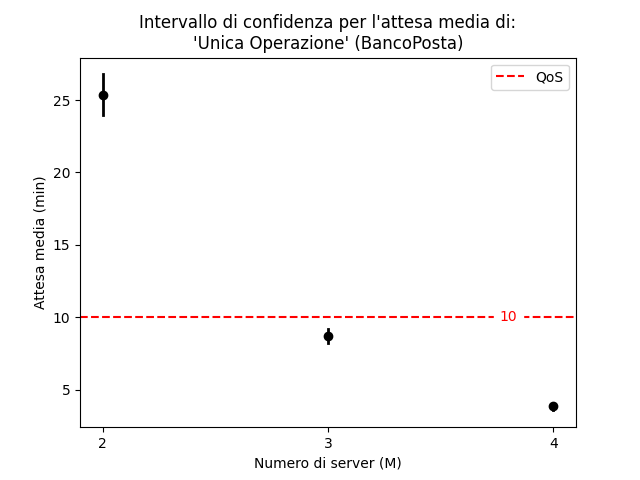
\includegraphics[width=\textwidth]{plots/d0-trans-imp}
\caption{\uo{} BP}
\label{fig:miglioria-esperimenti-simulazione-1a}
\end{subfigure}
\hfill    
\begin{subfigure}[b]{0.475\textwidth}  
\centering 
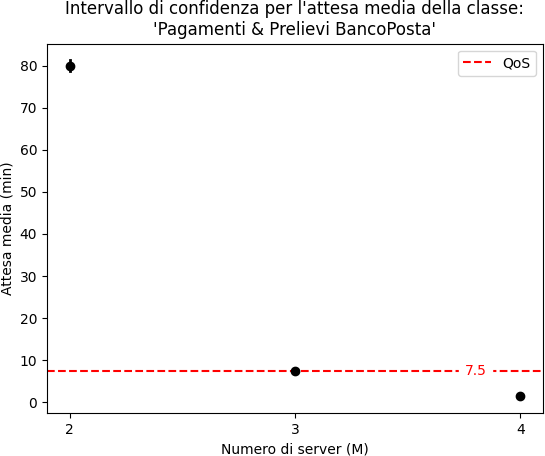
\includegraphics[width=\textwidth]{plots/d1-trans-imp}
\caption{\pp{} BP}
\label{fig:miglioria-esperimenti-simulazione-1b} 
\end{subfigure}

\vskip\baselineskip

\begin{subfigure}[b]{0.475\textwidth}   
\centering 
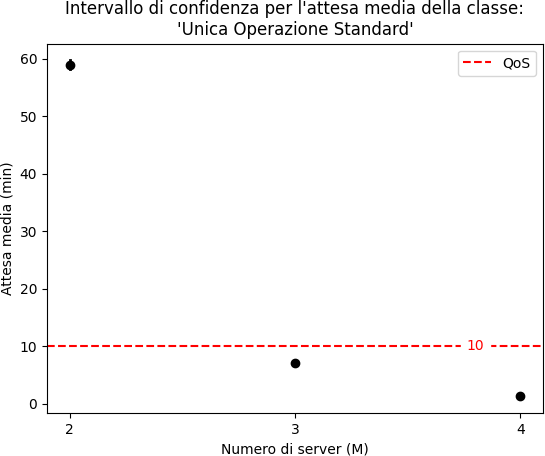
\includegraphics[width=\textwidth]{plots/d2-trans-imp}
\caption{\uo{} STD}
\label{fig:miglioria-esperimenti-simulazione-1c}
\end{subfigure}
\hfill
\begin{subfigure}[b]{0.475\textwidth}   
\centering 
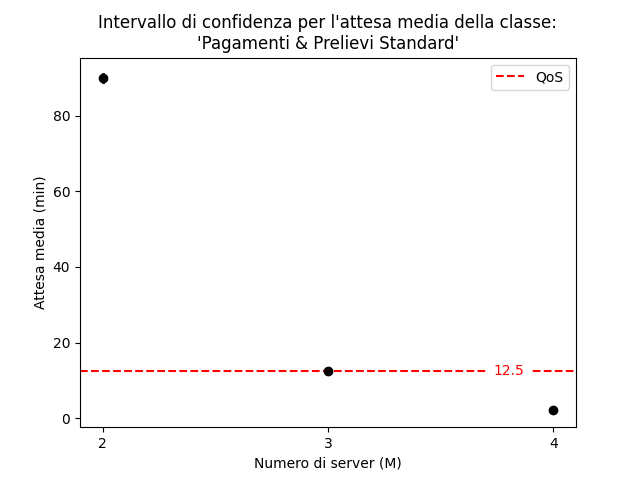
\includegraphics[width=\textwidth]{plots/d3-trans-imp}
\caption{\pp{} STD}
\label{fig:miglioria-esperimenti-simulazione-1d}
\end{subfigure}

\vskip\baselineskip

\begin{subfigure}[b]{0.475\textwidth}   
\centering 
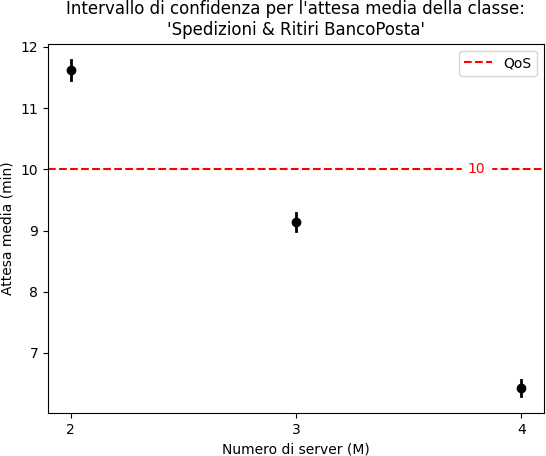
\includegraphics[width=\textwidth]{plots/d4-trans-imp}
\caption{\sr{} BP}    
\end{subfigure}
\hfill
\begin{subfigure}[b]{0.475\textwidth}   
\centering 
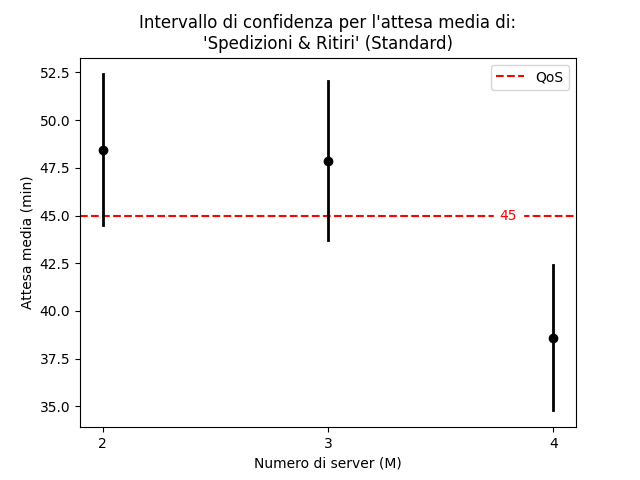
\includegraphics[width=\textwidth]{plots/d5-trans-imp}
\caption{\sr{} STD}    
\end{subfigure}
\caption{Attesa espressa in minuti, per ciascun flusso, al variare di $M$}
\label{fig:miglioria-esperimenti-simulazione-1}
\end{figure}